\chapter{GIỚI THIỆU VÀ MÔ TẢ BÀI TOÁN}
% \epigraph{\itshape  La volonté trouve, la liberté choisit. Trouver et choisir, c'est penser}{-- Victor Hugo}

\startcontents[chapters]
\printmyminitoc{
	Ghi 1 đoạn để tóm tắt nội dung chính trong chương. Phần Introduction phải giới thiệu được ngữ cảnh vấn đề từ chung--> cụ thể, nêu rõ motivation để thực hiện bài toán, giới thiệu tổng quát các đóng góp của nghiên cứu, và giới thiệu cấu trúc bài viết. (độ dài khoảng 20\% độ dài report).
}

\section{Giới thiệu}\label{sec:introduction}
\selectlanguage{vietnamese} 
Minh họa tham chiếu. Hình \ref{fig:f11} và  \ref{fig:f12} minh họa các trích dẫn. Các bạn truy cập vào link \footnote{https://www.doi2bib.org/} để lấy script rồi dán vào file bib. Sau đó lấy nhãn để trích dẫn, chi tiết xem Hình \ref{fig:fall}. Vd: viết tham chiéu và trích dẫn: Các tác giả trong \cite{Liu2024} đã đề xuất phương pháp... để...

Bảng \ref{tab:data} thể hiện xyz....

\begin{table}[ht!]
\centering
\caption{Đây là bảng}\label{tab:data}
\begin{tabular}{|l|l|l|l|l|}
\hline
a  & d & d & d & d \\ \hline
12 & 2 & 3 & 3 & 3 \\ \hline
\end{tabular}
\end{table}

Đây là ví dụ tham chiếu hình. Hình \ref{fig:hinh1} minh họa logo Google.
\begin{figure}[!ht]
    \centering
    
\includegraphics[width=0.45\textwidth]{images/assets/zgo.jpg}
    \caption{Vi du trinh bay 1 hinh.}
    \label{fig:hinh1}
\end{figure}
    
\begin{table}[ht!]
    \centering
    \caption{Vi du trinh bay 1 table.}\label{tab:img_para}
    \begin{tabular}{|l|r|r|r|}
        \hline 
        \textbf{No.}& \textbf{Size}&	\textbf{Number of cuts} &	\textbf{Total cube}\\
       \hline
        1   &	    32x32x32   &(8, 8, 5)     &320\\
        \hline
        2   &	    16x16x16   &(15, 15, 10)     &2050\\  
        \hline
    \end{tabular}
\end{table}

\begin{figure}[ht!]
\centering
\begin{subfigure}{0.495\textwidth}
    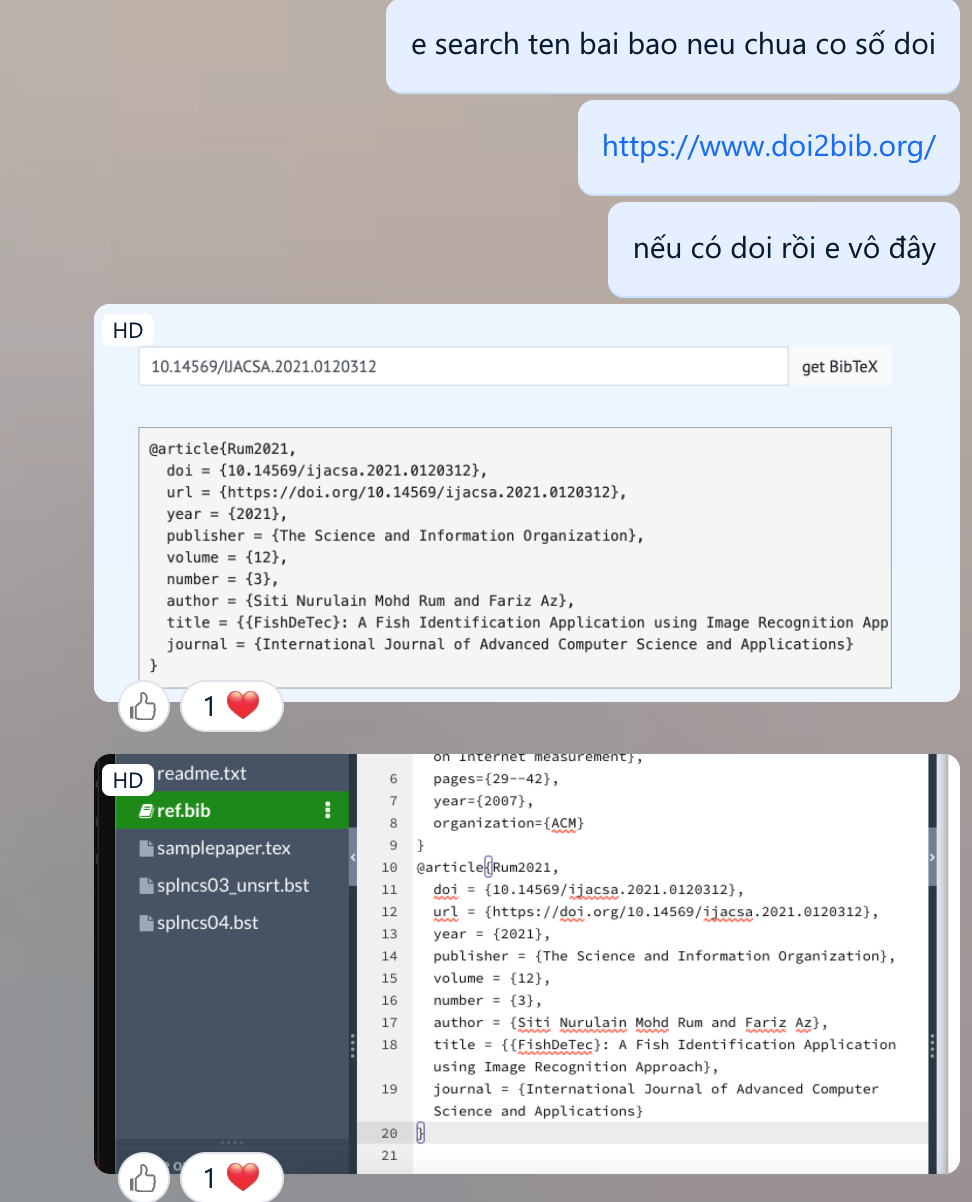
\includegraphics[width=\textwidth]{images/assets/zb1.png}
    \caption{Buoc 1.}
    \label{fig:f11}
\end{subfigure}
\hfill
\begin{subfigure}{0.495\textwidth}
    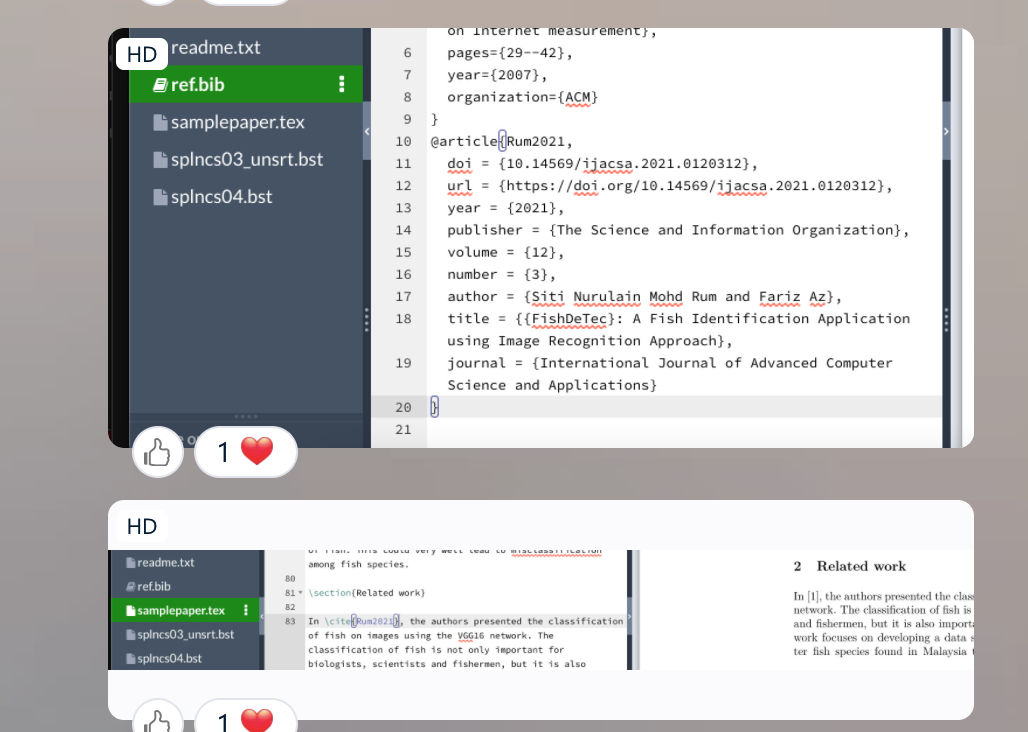
\includegraphics[width=\textwidth]{images/assets/zb2.png}
    \caption{Buoc 2}
    \label{fig:f12}`
\end{subfigure}
\caption{Hướng dẫn cách trích dẫn}
\label{fig:fall}
\end{figure}

\section{Các đóng góp chính của nghiên cứu}

\chapter{Các nghiên cứu có liên quan}
\printmyminitoc{
	Ghi 1 đoạn để tóm tắt nội dung chính trong chương. Mỗi bài đưa vào phải nhận xét về pp của họ, kq họ đạt được, điểm mạnh điểm yếu. Có thể phân nhóm các pp lại để viết cho mạch lạc nhất (độ dài khoảng 20\% độ dài report).
}
\section{Hướng nghiên cứu 1}
Trong nghiên cứu \cite{Shelke2021}, các tác giả đã....
\section{Hướng nghiên cứu 2}
\section{Hướng nghiên cứu 3}
\chapter{THIẾT KẾ VÀ CÀI ĐẶT GIẢI PHÁP}

\startcontents[chapters]
\printmyminitoc{
	Tóm tắt nội dung chính trong chương.
}
\section{Kiến trúc tổng quát hệ thống}
Kiến trúc (luồng xử lý tổng thể) của hệ thống đề xuất:  trước tiên trình bày sơ đồ workflow của pp đề xuất, giới thiệu các thành phần bên trong sơ đồ nhằm mục đích gì để thực hiện bài toán, các mô hình dữ liệu.... Các thành phần này sẽ chia thành các mục Subsection để giải thích rõ các thành phần (độ dài khoảng 20-30\% độ dài report)

\section{Thu thập dữ liệu}
Mô tả chi tiết dữ liệu dùng cho thực nghiệm (độ phân giải ảnh, số lớp, số sample, số sample mỗi phân lớp, nguồn download, các bài toán/nghiên cứu đã dùng dữ liệu này (nếu dùng các dữ liệu được public)....)

\section{Mô tả thành phần 1 trong kiến trúc tổng quát}
Mô tả chi tiết từng thành phần con trong workflow.
\section{Mô tả thành phần 2 trong kiến trúc tổng quát}
Mô tả chi tiết từng thành phần con trong workflow.

\chapter{KIỂM THỬ VÀ ĐÁNH GIÁ}
\startcontents[chapters]
\printmyminitoc{
	Tóm tắt nội dung chính trong chương.
}

\section{Môi trường cài đặt và cách đánh giá}
\subsection{Thiết lập môi trường thực nghiệm}

\subsection{Các độ đo đánh giá}
Cần liệt kê rõ các độ đo sử dụng, bao gồm các công thức và ý nghĩa thành phần trong công thức.

Ví dụ: Công thức tính độ chính xác như được trình bày trong Công thức \ref{eq:acc}.



\begin{equation}\label{eq:acc}
Accuracy = \frac{TP+TN}{TP+TN+FP+FN}   
\end{equation}

\begin{equation}
Precision = \frac{TP}{TP+FP}
\end{equation}

\begin{equation}
Recall = \frac{TP}{TP+FN}
\end{equation}

\begin{equation}
F1 = \frac{2*Precision*Recall}{Precision+Recall} = \frac{2*TP}{2*TP+FP+FN}
\end{equation}
\section{Kết quả phương pháp đề xuất}
Nhận xét kết quả đặc sắc/thú vị tìm thấy trong nghiên cứu. Cần trình bày đủ các độ đo nhất có thể (accuracy, f1-score, confusion matrix, AUC, MCC,... cho bài toán phân lớp, IoU, Dice,... cho bài toán phân vùng, và các độ khác tương ứng với bài toán) gồm kết quả trên tập Train/Test (và Validation nếu có)

\subsection{Kịch bản 1}
\subsection{Kịch bản 2}
\subsection{Kịch bản 3}
\section{Thảo luận kết quả và so sánh kết quả so với các phương pháp trước đó}
\section{Giới thiệu chương trình cài đặt từ phương pháp đề xuất}
\subsection{Giới thiệu chương trình để huấn luyện mô hình}

\subsection{Giới thiệu chương trình triển khai mô hình máy học đã huấn luyện}

\chapter{KẾT LUẬN VÀ HƯỚNG PHÁT TRIỂN}
\startcontents[chapters]
Kết luận (những kết quả chung đạt được, những kiến thức đã tiếp nhận được,....) và hướng phát triển.
\section{Kết luận}
\section{Hướng phát triển}
